\section{Object Detection and Instance Segmentation}

\subsection{任务简介}

\begin{figure}[htbp]
    \centering
    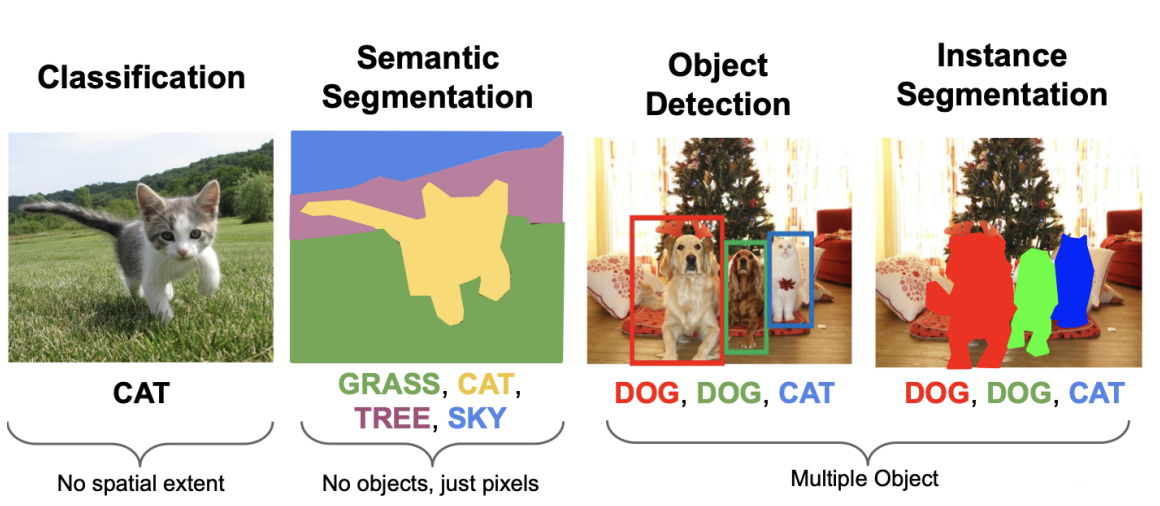
\includegraphics[scale=0.55]{figures/cv_tasks.png}
    \caption{分类任务}
\end{figure}

如上的任务当中,最左侧的是分类,即一张图片里只有一个待分类的事物.随后是语义分割,即将代表不同语义的像素区分开来,每个像素都要有一个输出,它不区分不同的个体.随后是目标检测,它区分不同个体,但并不一定每个像素都被一个bounding box包围.最后在此之上可以继续进行语义的分割.

我们先从Object Detection中最简单的Single Object说起.它的目标是定位和分类,网络输出是2D的bounding box,且是axis aligned的.\footnote{到了三维的时候,由于阶数的提升,axis-aligned bounding box中有非常多的部分并不属于这个物体,因此可能需要旋转.但是对2D来说,这并不成为问题.}确定bounding box需要四个参数$x, y, w, h$,即bbox左上角的坐标和大小.\footnote{如果我们用八个点的坐标作为表示,那么显然有很多冗余.尤其在高维的情形,如何找到冗余尽可能少而能够便利地表达某一对象的方法是非常重要的.在后面的旋转部分,我们还会看到这一点.}

总的来说,单目标检测可以被划分成两个任务:(对图片的)\textbf{分类}和(对bbox)的\textbf{回归}.如下图:

\begin{figure}[htbp]
    \centering
    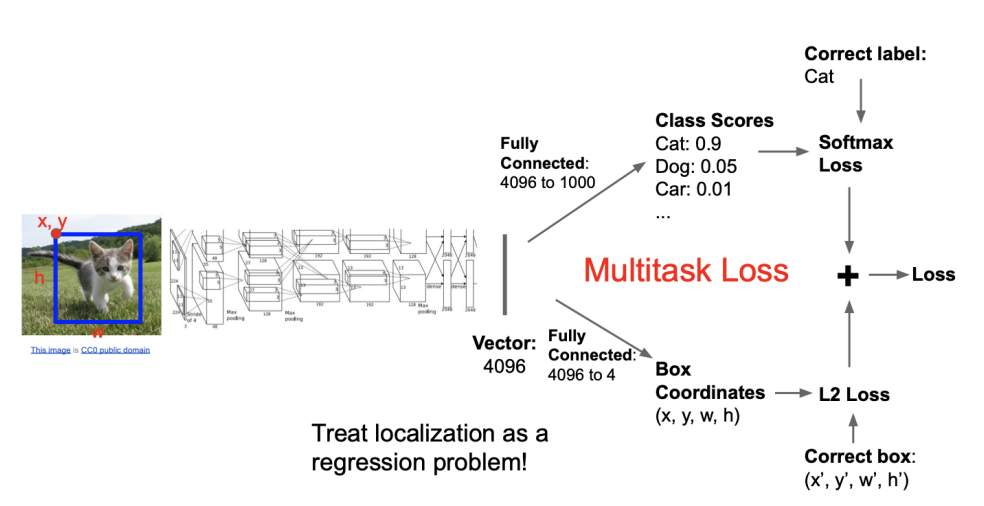
\includegraphics[scale=0.55]{figures/single_obj_det.png}
    \caption{单目标检测的网络概念图}
\end{figure}

假设我们得到了图片的特征向量,那么可以通过MLP变成分类概率的向量,然后使用交叉熵进行度量;然后我们对图片MLP到四个数值,然后用$L^2$ loss进行回归\footnote{注意$L^2$ norm和$L^2$ loss的区别.前者是模长,后者是平方和.当$L^2$ norm作为损失函数时,被称为rooted mean squared error(RMSE),而另一个则是mean squared error.L2在接近收敛的时候,梯度也小,不容易越过.但是L2在较大的时候,梯度很大,容易导致神经网络训练效果不好,而且还容易出现NaN.RMSE因为开根号的问题,在接近收敛时反而可能出现问题.soft L1:结合两者.}.

这是一个Multitask Loss,即分类loss和bounding box的loss之和,可能产生竞争.它们应该以何种比例叠加?比如分类的loss最大大概在$\log N$的量级,但是对bounding box来说,如果采用$L^2$,差5个pixel那就是25.而$e^{25}$是一个非常大的数字.即使loss的量级差不多,gradient的量级也不一定是相同的.

除此之外,这个网络还有一个特殊性质:对于不同图片,可能需要不同数量的输出.这在以前的Neural Network是无法做到的.传统的方法是用sliding window进行遍历检测,但这也自然而然带来一个问题:你怎么知道window多大呢?后来的传统方法采用了Region Proposal的方法,即先提出一些可能是物体的bbox,在其中进行检测.后来将这些proposal称为Region of Interest(RoI).
\subsection{Region-based CNN}

第一个深度学习的相关工作\cite{RCNN}:R-CNN(Region-based CNN).它的大致流程是:先提出一些proposal,然后通过SVM进行分类,以及对bbox的回归,回归的输出是$(dx, dy, dh, dw)$,即bbox应该进行的调整.为了处理不同大小的bbox输入,RCNN将所有的bbox覆盖的部分统一变换到224*224的大小.

\begin{figure}[htbp]
    \centering
    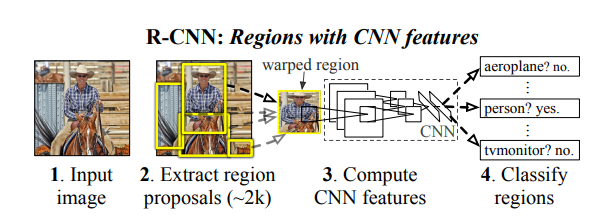
\includegraphics[scale=0.7]{figures/RCNN_classification.png}
    \caption{RCNN分类部分}
\end{figure}

训练时我们会有很多的RoI,但ground truth(后文简写成gt)的数量显然要少得多.那么如何确定一个RoI被分成哪一类,以及向哪个gt进行回归呢?首先,如果一个bbox与任何一个gt的交都小于某一阈值,那么就将它单独分类成background,此时我们不再关心其regression的情况;如果一个bbox同时包含了多个gt,那么可以计算它与这些gt的IoU,将IoU最大的那个gt作为其分类和回归的对象.这里要注意的是,我们不关注background的回归是必须采取的行为,因为如果要监督一个background的回归,那么它的loss是非常大的,会直接破坏其他RoI的训练.

这个工作的两个问题:首先proposal可能太多了,在测试时速度太慢.其次若给出的proposal可能有缺损,将其单独提取出来之后的部分无法获知周围的信息,几乎不可能准确对bbox进行回归.

\subsection{Fast R-CNN}


\begin{figure}[htbp]
    \centering
    \subfigure[取对应的bbox]{
        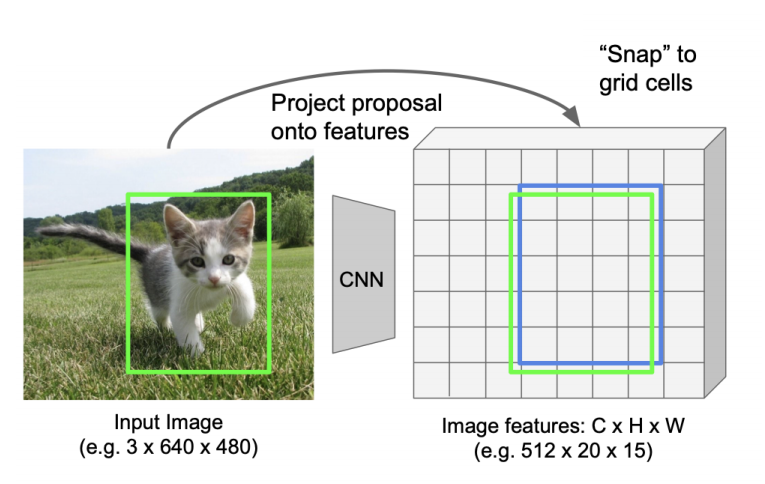
\includegraphics[scale=0.45]{figures/RoI_pool.png}
        \label{fig:get bbox in feature map}
    }
    \subfigure[RoI pool]{
        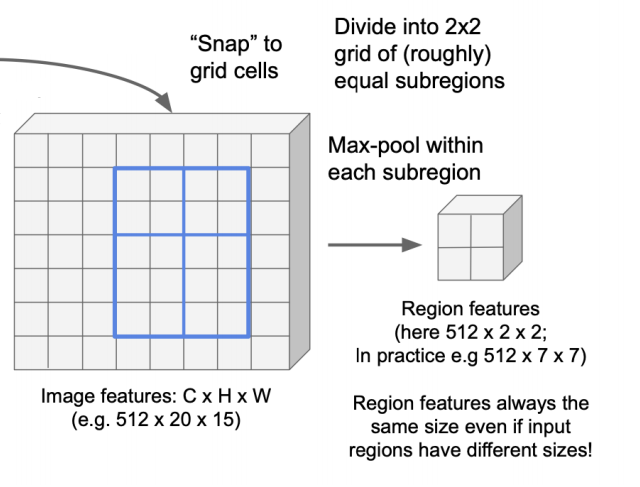
\includegraphics[scale=0.45]{figures/RoI_pool2.png}
        \label{fig:RoI_pooling}
    }
    \caption{Fast RCNN}
\end{figure}

随后提出的Fast R-CNN解决了上面的两个问题.Fast RCNN仍然采用传统方法获得RoI,随后将整个图片过CNN,再在feature map上取出对应的bbox.图像在卷积的过程中分辨率会减小,因此在feature map上取的时候也要对应地缩小RoI,如图 \ref{fig:get bbox in feature map}所示,缩小过程中不在格点上的顶点被吸附到最近邻的格点上.

这样取得的RoI大小仍然不统一,原论文采用了一种max pooling的方法,将形式各异的RoI分割成合乎要求的子块,对每个子块求最大值获得期望的形状,如图 \ref{fig:RoI_pooling}所示.图中为方便将最终的大小画成了2*2,实际上为7*7.

这样做的好处是,可以将多出来的RoI数量这一维度作为Batch的一部分,从而实际上并不会明显扩大工作量,因为最后的RoI分辨率比较小.以7*7为例,1000个RoI总共约50k个数据,与224*224大小的原图相仿.另外,经过conv后,感受野也增大了,也就不会产生上文提到的被裁剪而缺少上下文的问题了.Fast RCNN相比RCNN取得了可观的速度提升.下图左侧,Fast RCNN的训练时间只有RCNN的约十分之一,且测试速度显著提高.右图红色为不包含传统方法获得RoI,仅对RoI进行处理的时间,可以看出时间的限制在RoI的提出上了.

\begin{figure}[htbp]
    \centering
    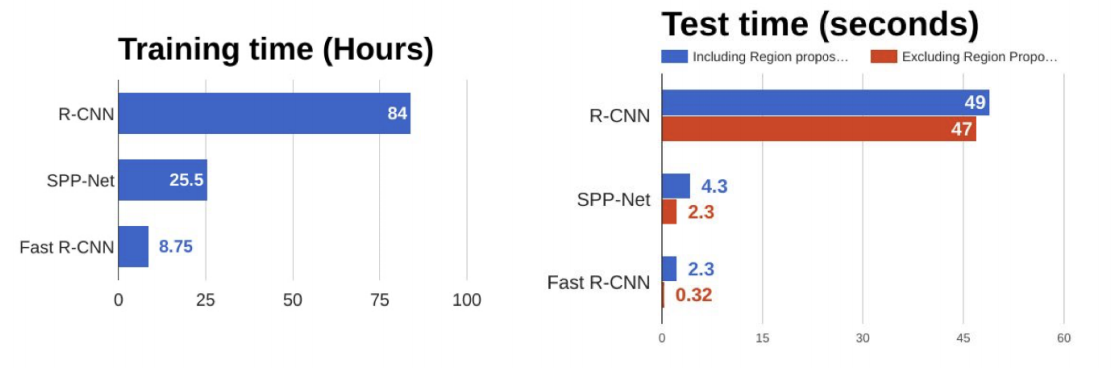
\includegraphics[scale=0.65]{figures/rcnn_vs_frcnn.png}
    \caption{RCNN v.s. Fast RCNN}
    \label{}
\end{figure}

\subsection{Faster R-CNN}

经过R-CNN和Fast R-CNN的积淀,Ross B. Girshick在2016年提出了新的Faster RCNN.在结构上,Faster RCNN已经将特征抽取(feature extraction),proposal提取,bounding box regression,classification都整合在了一个网络中,使得综合性能有较大提高,在检测速度方面尤为明显.

\begin{wrapfigure}{l}{4cm}
    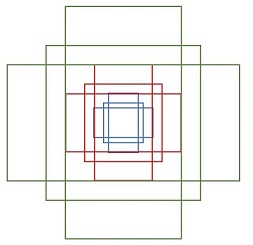
\includegraphics[scale=0.5]{figures/anchor.jpg}
    \caption{不同形状的anchor}
    \label{fig:anchor}
\end{wrapfigure}

Faster R-CNN引入Anchor box的概念.在Fast R-CNN中,我们已经得到了feature map,而其中的每个pixel都可能含有不同形状的一个或多个物体,直接将取每个pixel作为RoI是不合理的.Faster R-CNN让每个pixel都给出一些不同形状的anchor(如图 \ref{fig:anchor}所示).这个部分被称为Region Proposal Network(RPN).

当然,这样会获得数千个乃至更多的bbox,而一张图片里一般并没有这么多,而这里我们并没有gt可供参考,因此我们还要进行NMS.具体来说,先将这些bbox进行分类预测,按照它们的分类进行分组,随后对每个类型的分组内取分类概率最高的RoI,将同组之内和它IoU大于某个threshold的RoI全部去除.这样做的原理是将某一类别概率最高的作为标准,与其IoU较大的则认为是圈出了同一个物体,全部去除;对于剩余的RoI重复这一操作.\footnote{举例来说,假设猫分类的RoI中概率最大者圈住了一只猫的绝大多数,因而以90\%的confidence认为是猫,则其他与它IoU大于0.5的RoI很可能只圈住了这只猫的半边身子,所以把它们都去掉.而IoU较小的可能是其他的猫.当然,这样做也存在一些问题,比如有一个和它非常接近的RoI因为某种原因识别为狗,那么这样做就不能去除这样的RoI,因为此处NMS只对同类的RoI进行操作.后来也有工作同时预测RoI与IoU(即"预测的预测"),并证明这样做效果更优.}

\begin{wrapfigure}{r}{6cm}
    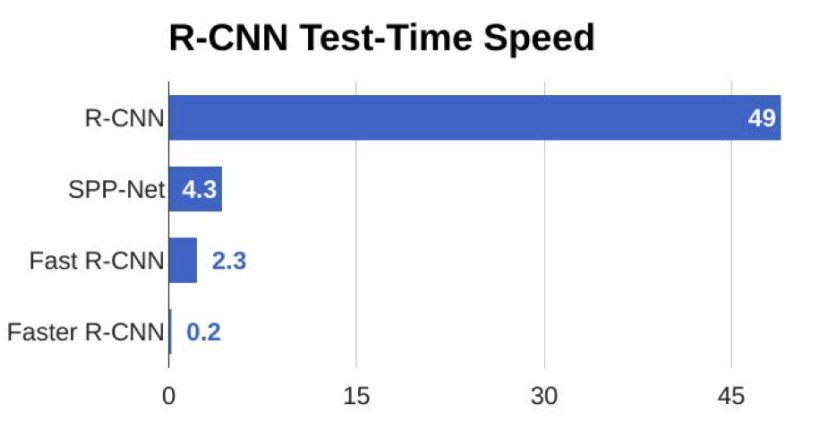
\includegraphics[scale=0.4]{figures/rcnn_speed_comparison.png}
    \caption{几种网络的速度比较}
    \label{fig:rcnn_speed}
\end{wrapfigure}

当然,Faster R-CNN之中还有非常多的细节,比如anchor如何取定,如何确定训练RPN的positive/negative samples,如何参数化bbox回归的过程等,限于篇幅限制无法一一展开,读者可参考\cite{FasterRCNNzh=cn}.

Faster R-CNN中包含了四种loss:RPN对是否是物体的二分loss,RPN regress box loss, final classification score, final box coordinates, 调参的过程自然是非常复杂的,但是网络的效果也是显而易见的(如图 \ref{fig:rcnn_speed}).Faster R-CNN的出现,使得目标检测不再是学术界的toy model, 而是真正进入了实用领域,促进了安保等行业的发展.

\subsection{two-stage detector and one-stage detector}

\begin{figure}[htbp]
    \centering
    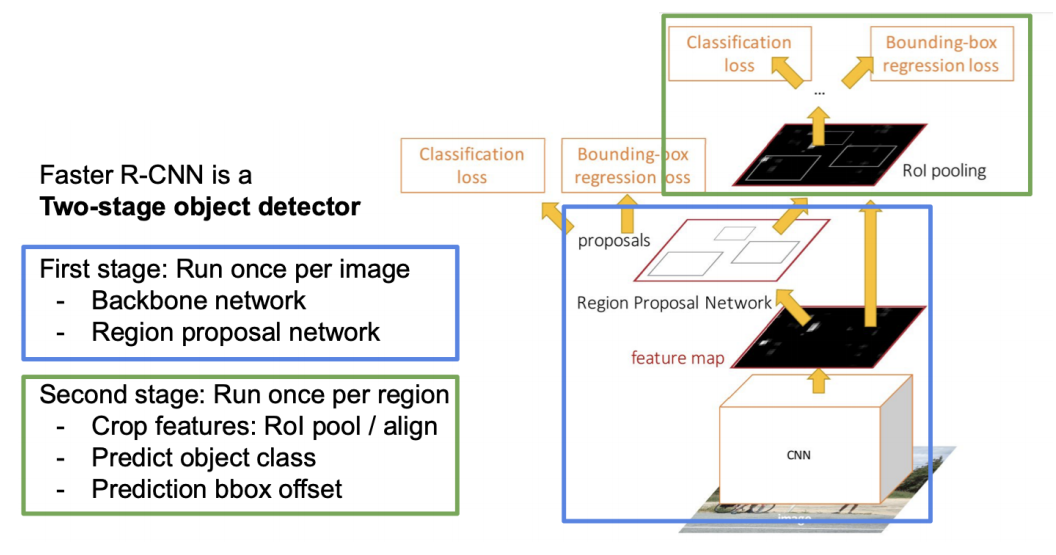
\includegraphics[scale=0.45]{figures/two_stage_detector.png}
    \caption{Two Stage示意}
    \label{}
\end{figure}

如上图,Faster R-CNN是一个分两步的目标检测网络.有人提出:既然在第一步里也做了bbox 的refine,那么能否去掉第二步呢?这就诞生了single-stage detectors,代表有YOLO系列,它的特点就是非常快,目前能达到120 fps.总体来说,two stage准确率占优,而one stage速度更快.

\subsection{Evaluation Metric: mAP}

无论是一步还是两步,都需要面临的问题:我们如何评估预测结果?\marginpar{\kaishu 这是边注.这段话测试一下边注的分段和位置.
    
庾信平生最萧瑟,暮年诗赋动江关.$$a = b$$}假如我们有一张图,有20个ground truth bounding box,我们显然不可能要求其完全相符.我们可以定义一个IoU threshold.首先其输出的类别要对,其次IoU>threshold.另外一方面,如果我乱猜了5000张,显然也是不行的.trade-off between recall \& precision.因此提出度量:AP.即Average Precision.即precision-recall图像下的面积.它先选出某个种类,然后按照prob排序,逐个增加.这样precision下降,recall提升.mAP就是所有不同category and/or IoU threshold.

Object detection变量非常多.若要准确度,则Faster R-CNN.若要快速:YOLO.但目前这一领域,工业界已经占据了统治地位.
